\subsection{Data loading and preprocessing}\label{sec:data loading and preprocessing}
In order to load the data, we use the Pandas library for Python.
Data are loaded from CSV files and then passed to the preprocessing stage.

Preprocessing is done by first stripping the Pandas DataFrame of all columns except the target column $y$. In our case, this is the column denoting the temperature.

Next, we add $n$ time lag features. Let $x_{t,y}$ denote value of the target attribute $y$ at time step $t$ for $N$ sensors. 
Time lag features are added by adding $L=\{1,\dots, n\}$ attributes where $L_{i=1}^n=x_{t-i, y}$ for each $x_{t}$.```

As we used different Python frameworks for different models, the processing from here depended on the framework. Some models required the dataset to be converted to tensors, and others did not.
Besides this, we also split the data into test and training sets with a $0.33/0.77$ distribution for testing and training, respectively.

The point of transformers was to overcome the problems faced by the previous state-of-the-art architectures while still including prominent aspects of the RNN and Convolutional Neural Network (CNN) models.

The RNN model has two notable weaknesses. First is its inability to learn long-term patterns, due to the exploding and vanishing gradient problems that occur during backpropagation.
Secondly, its recurrent connection is also a weakness. This is because it is not possible to compute the cell at time step $i$ until the cell at time step $i-1$ has been computed as information is propagated along a sequence.

In contrast, one of the benefits of CNNs is that they can be computed concurrently. However, unlike RNNs, they are unable to learn even short-term patterns. The size of the patterns they can learn is limited by their architecture.

Transformers attempt to feature the best of both techniques.
Transformers can model dependencies over the whole range of the input sequence as easily they can model neighboring sequences. And there are no recurrent connections, allowing efficient computation using parallelization. This is facilitated through the use of the self-attention mechanism.\cite{TransformersScratchPeterbloem}

\begin{figure}[h]
  \centering
  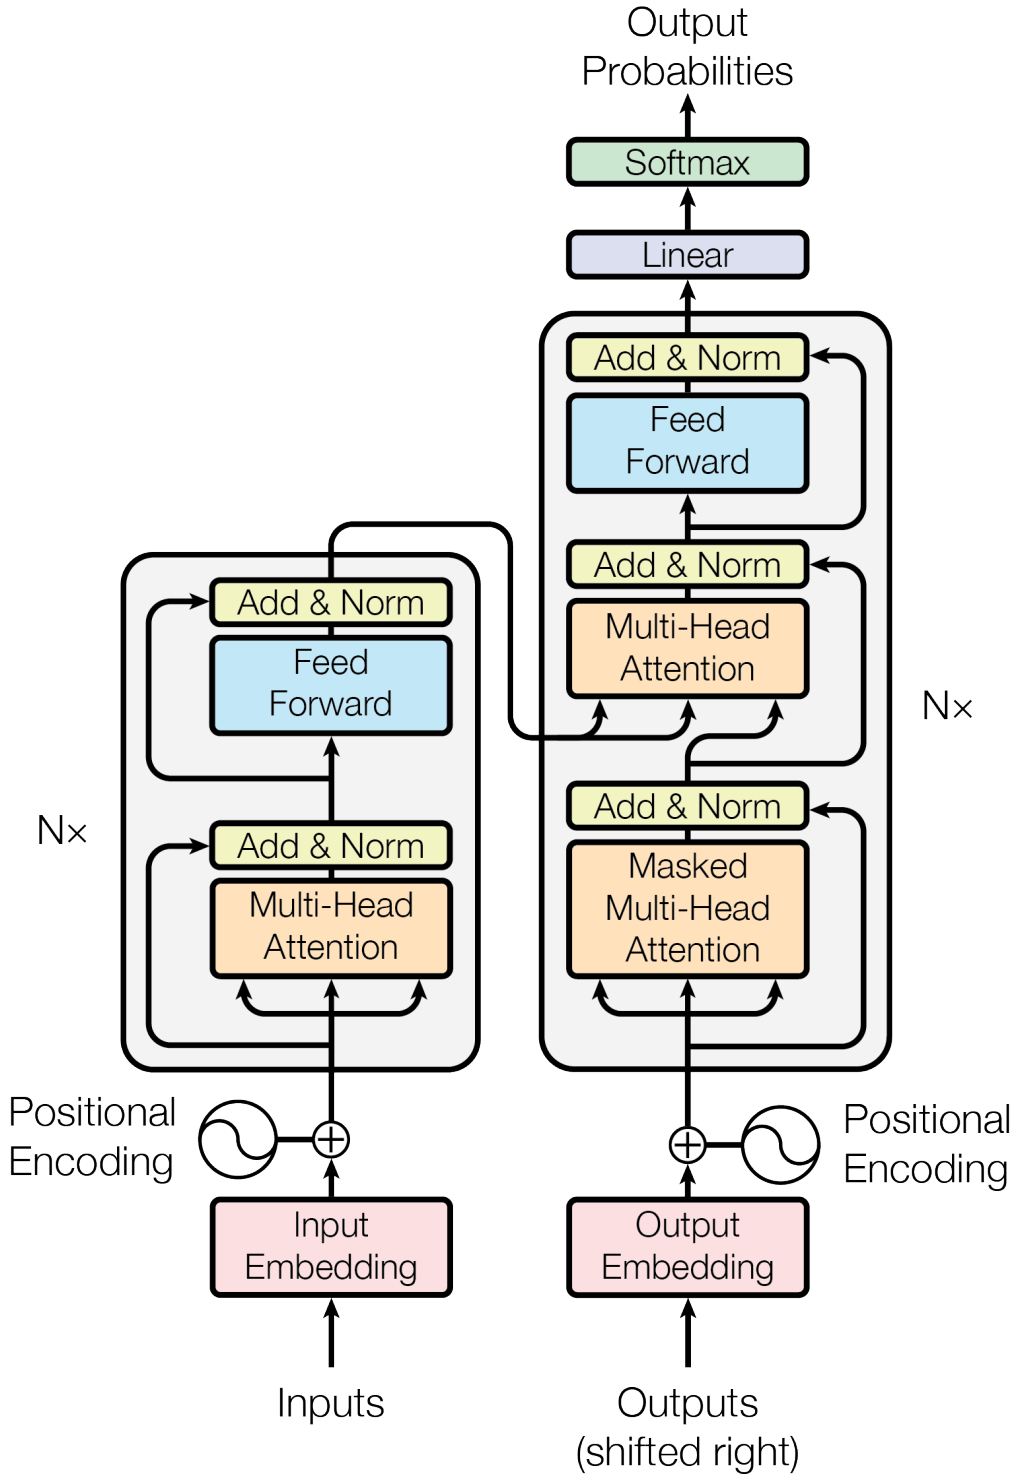
\includegraphics[width=0.5\textwidth]{Transformer model diagram}
  \caption{Diagram depicting the architecture of the transformer model from \citet{AttentionIsAllYouNeed}.}
  \label{fig:original transformer}
\end{figure}